% !TeX program = lualatex
% ================================================================
% Polish Parallel Text Version of VectorsRacetrack
%
% Generated by the server using the following settings:
%
%   language            Polish (pol)
%   text direction      left to right
%   font                Noto Serif
%   fallback font       Noto Serif
%   built from          latex/worksheets/geometry/vectors/vectorsRacetrack.tex
%   vocabulary key      latex/worksheets/geometry/vectors/vectorsRacetrack/L2/pol/vectorsRacetrack_polishKey.tex
%   tier 3 vocabulary   green   RGB 0 128 0
%   English text        black   RGB 0 0 0
%   Polish text         purple  RGB 112 48 160
%   layout macros       version 3
%
% Please don't edit any information in this comment block - the server
% compares it against the current settings and rebuilds this file when
% they differ, so changes here would be overwritten. However, feel free
% to make updates to the LaTeX below if you want to edit it.
% ================================================================

\documentclass[12pt,a4paper]{article}
% ================================================================
% Copied from the English sheet this was translated from, so that
% anything it sets up for itself still works here
% ================================================================
\usepackage{amsmath, amssymb, tikz, geometry, tabularx}
\geometry{margin=1in}
\setlength{\parskip}{6pt}

\title{Vector Worksheet}
\author{}
\date{}

% Characters this language's font has not got are borrowed from another,
% rather than being silently dropped - see docs/translated-sheet-latex.md
\directlua{%
  if luaotfload and luaotfload.add_fallback then
    luaotfload.add_fallback("eallatinfallback",
      { "Noto Serif:mode=harf;" })
  else
    tex.error("this luaotfload is too old to register a fallback font")
  end
}
\usepackage[english]{babel}
\babelprovide[import]{polish}
\babelfont[polish]{rm}[Renderer=Harfbuzz, BoldFont={Noto Serif}, ItalicFont={Noto Serif}, BoldItalicFont={Noto Serif}, RawFeature={fallback=eallatinfallback}]{Noto Serif}
\babelfont[polish]{sf}[Renderer=Harfbuzz, BoldFont={Noto Serif}, ItalicFont={Noto Serif}, BoldItalicFont={Noto Serif}, RawFeature={fallback=eallatinfallback}]{Noto Serif}
\newcommand{\ealtext}[1]{\foreignlanguage{polish}{#1}}
\newcommand{\ealtextblock}[1]{{\raggedright\foreignlanguage{polish}{#1}\par}}
% ================================================================
% EAL layout helpers
% ================================================================
\usepackage{xcolor}

\definecolor{ealkeycolour}{RGB}{0,128,0}
\definecolor{ealenglish}{RGB}{0,0,0}
\definecolor{ealtwocolour}{RGB}{112,48,160}

\newsavebox{\ealboxen}
\newsavebox{\ealboxtr}
\newlength{\ealglosswd}
\newlength{\ealglossraise}
\setlength{\ealglossraise}{1.15em}

% a tier 3 word, in English and in translation alike
\newcommand{\ealkey}[1]{\textcolor{ealkeycolour}{#1}}
\newcommand{\ealkeytr}[1]{\textcolor{ealkeycolour}{\ealtext{#1}}}

% One translated word above one English word. Built from kernel
% primitives, never a tabular, which would break wherever the sheet
% loads array, booktabs or tabularx. The box is as wide as the wider of
% the two, so a long translation pushes its neighbours aside instead of
% overlapping them, and it claims its full height so a table row or a
% TikZ node makes room for it.
\newcommand{\ealgloss}[2]{%
  \sbox{\ealboxen}{\ealkey{#1}}%
  \sbox{\ealboxtr}{\small\textcolor{ealtwocolour}{\ealtext{#2}}}%
  \setlength{\ealglosswd}{\wd\ealboxen}%
  \ifdim\wd\ealboxtr>\ealglosswd\setlength{\ealglosswd}{\wd\ealboxtr}\fi
  \leavevmode
  \makebox[\ealglosswd][c]{%
    \makebox[0pt][c]{\usebox{\ealboxen}}%
    \makebox[0pt][c]{\raisebox{\ealglossraise}{\usebox{\ealboxtr}}}%
  }%
}

% opens up line spacing around a block of glosses, so the raised
% translations sit clear of the line above
\newenvironment{ealglossed}{\par\linespread{2.1}\selectfont\ignorespaces}{\par}

% a whole translated sentence above its English counterpart. block level,
% so it does not belong inside a tabular cell
\newcommand{\ealpara}[2]{%
  \par\addvspace{0.5\baselineskip}%
  {\color{ealtwocolour}\ealtextblock{#1}}%
  \penalty200
  {\color{ealenglish}#2\par}%
  \addvspace{0.5\baselineskip}%
}

\begin{document}
\maketitle
\thispagestyle{empty}

\ealpara{Przedstawienia \ealkeytr{wektorów}}{\ealkey{Vector} Representations}
\section*{\ealkey{Vector} Representations}

\ealpara{Użyj diagramu i częściowo wypełnionej tabeli, aby uzupełnić \textbf{trzy przedstawienia} dla każdego \ealkeytr{wektora}: (i) zmienną algebraiczną (zwykle pogrubioną) \( \mathbf{v}\), (ii) \ealkeytr{ścieżkę skierowaną} \( \overrightarrow{AB}\), (iii) \ealkeytr{wektor kolumnowy}.}{Use the diagram and the partially completed table to fill in the \textbf{three representations} for each \ealkey{vector}: (i) algebraic \ealkey{variable} (usually bold) \( \mathbf{v}\), (ii) \ealkey{directed path} \( \overrightarrow{AB}\), (iii) \ealkey{column vector}.}
\[
\text{(i)  algebraic variable (usually bold)  \( \mathbf{v}\),\quad }
\text{(ii)  directed path  \( \overrightarrow{AB}\),\quad }
\text{(iii) column vector }
\begin{pmatrix} x \\ y \end{pmatrix}.
\]

\ealpara{W ostatnich kolumnach utwórz własne przykłady.}{For the last columns, create examples of your own.}

\ealpara{W tabeli: punkty, \ealkeytr{ścieżka skierowana}, \ealkeytr{wektor kolumnowy}.}{In the table: points, \ealkey{directed path}, \ealkey{column vector}.}

\begin{center}
\small
\begin{tabularx}{\textwidth}{|>{\raggedright\arraybackslash}p{2cm}|>{\centering\arraybackslash}p{2cm}|>{\centering\arraybackslash}p{2cm}|>{\centering\arraybackslash}p{2.2cm}|>{\centering\arraybackslash}p{2.2cm}|}
\hline
& \textbf{\(\mathbf{u}\)} & \textbf{\(\mathbf{v}\)} & \textbf{\underline{\hspace{1.6cm}} } & \textbf{\underline{\hspace{1.6cm}} } \\
\hline

\textbf{Points } 
&
\(\;A = (0,0) \newline B = (3,-1) \)
&
\(\;P(2,3) \newline Q = (\underline{\hspace{0.8cm}})\)
&
\(\;C = (-3,2) \newline D = (1,5)\)
&
\(\;X = (5,0) \newline \underline{\hspace{0.5cm}} = (\underline{\hspace{0.8cm}})\)
\\
\hline

\textbf{\ealkey{Directed path}}
&
\( \newline \overrightarrow{AB} \)
&
\(\newline \overrightarrow{\boxed{\phantom{aaa}}} \)
&
\(\newline \overrightarrow{\boxed{\phantom{aaa}}} \)
&
\(\newline \overrightarrow{\boxed{\phantom{aaa}}} \)
\\
\hline



\textbf{\ealkey{Column vector}}
&
\(\begin{pmatrix} 3 \\ -1 \end{pmatrix}\)
&
\(\begin{pmatrix} 5 \\ 3 \end{pmatrix}\)
&
\(\begin{pmatrix}
\underline{\hspace{0.5cm}} \\[4pt]
\underline{\hspace{0.5cm}}
\end{pmatrix}\)
&
\(\begin{pmatrix}
\underline{\hspace{0.5cm}} \\[4pt]
\underline{\hspace{0.5cm}}
\end{pmatrix}\)
\\
\hline
\end{tabularx}
\end{center}

\vspace{0.5cm}

\ealpara{Dodawanie \ealkeytr{wektorów}.}{Adding \ealkey{vectors}.}
\section*{Adding \ealkey{vectors}}

\ealpara{Użyj podanych \ealkeytr{wektorów}, aby znaleźć trasę przez tor, która przecina linię mety; nie możesz opuścić szarego toru, ale możesz dotykać boków.}{Use the \ealkey{vectors} provided to find a route through the track, that crosses the finish line, you may not leave the grey track, but can touch the sides.}

---

\ealpara{\ealkeytr{Wektory}:}{\ealkey{Vectors}:}

\[
\begin{aligned}
\mathbf{a} &= \begin{pmatrix} 3 \\ 2 \end{pmatrix}, &
\mathbf{b} &= \begin{pmatrix} -3 \\ 2 \end{pmatrix}, &
\mathbf{c} &= \begin{pmatrix} 2 \\ -4 \end{pmatrix}, &
\mathbf{d} &= \begin{pmatrix} -2 \\ -3 \end{pmatrix}, \\[6pt]
\mathbf{e} &= \begin{pmatrix} 2 \\ -1 \end{pmatrix}, &
\mathbf{f} &= \begin{pmatrix} -4 \\ -1 \end{pmatrix}, &
\mathbf{g} &= \begin{pmatrix} 1 \\ 3 \end{pmatrix}, &
\mathbf{h} &= \begin{pmatrix} -1 \\ 4 \end{pmatrix}
\end{aligned}
\]

\begin{center}
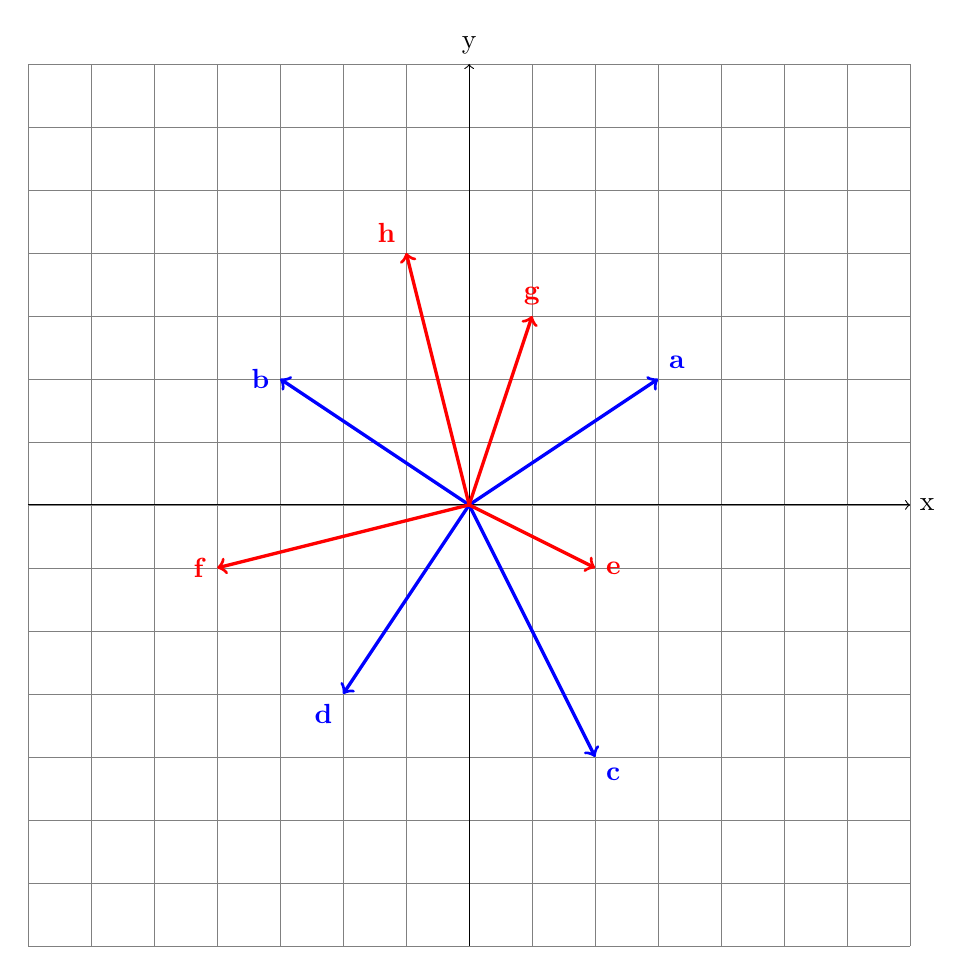
\begin{tikzpicture}[scale=0.8]

    % Grid + axes
    \draw[help lines, step=1] (-7,-7) grid (7,7);
    \draw[->] (-7,0) -- (7,0) node[right] {x};
    \draw[->] (0,-7) -- (0,7) node[above] {y};

    \tikzset{vec/.style={->, very thick}}

    % New varied vectors
    \draw[vec,blue] (0,0) -- (3,2)   node[midway, below right]{} node[above right]{\(\mathbf{a}\)};
    \draw[vec,blue] (0,0) -- (-3,2)  node[midway, above left]{} node[left]{\(\mathbf{b}\)};
    \draw[vec,blue] (0,0) -- (2,-4)  node[midway, right]{} node[below right]{\(\mathbf{c}\)};
    \draw[vec,blue] (0,0) -- (-2,-3) node[midway, left]{} node[below left]{\(\mathbf{d}\)};

    \draw[vec,red]  (0,0) -- (2,-1)  node[midway, above right]{} node[right]{\(\mathbf{e}\)};
    \draw[vec,red]  (0,0) -- (-4,-1) node[midway, above left]{} node[left]{\(\mathbf{f}\)};
    \draw[vec,red]  (0,0) -- (1,3)   node[midway, right]{} node[above]{\(\mathbf{g}\)};
    \draw[vec,red]  (0,0) -- (-1,4)  node[midway, left]{} node[above left]{\(\mathbf{h}\)};

\end{tikzpicture}
\end{center}

---

\begin{center}
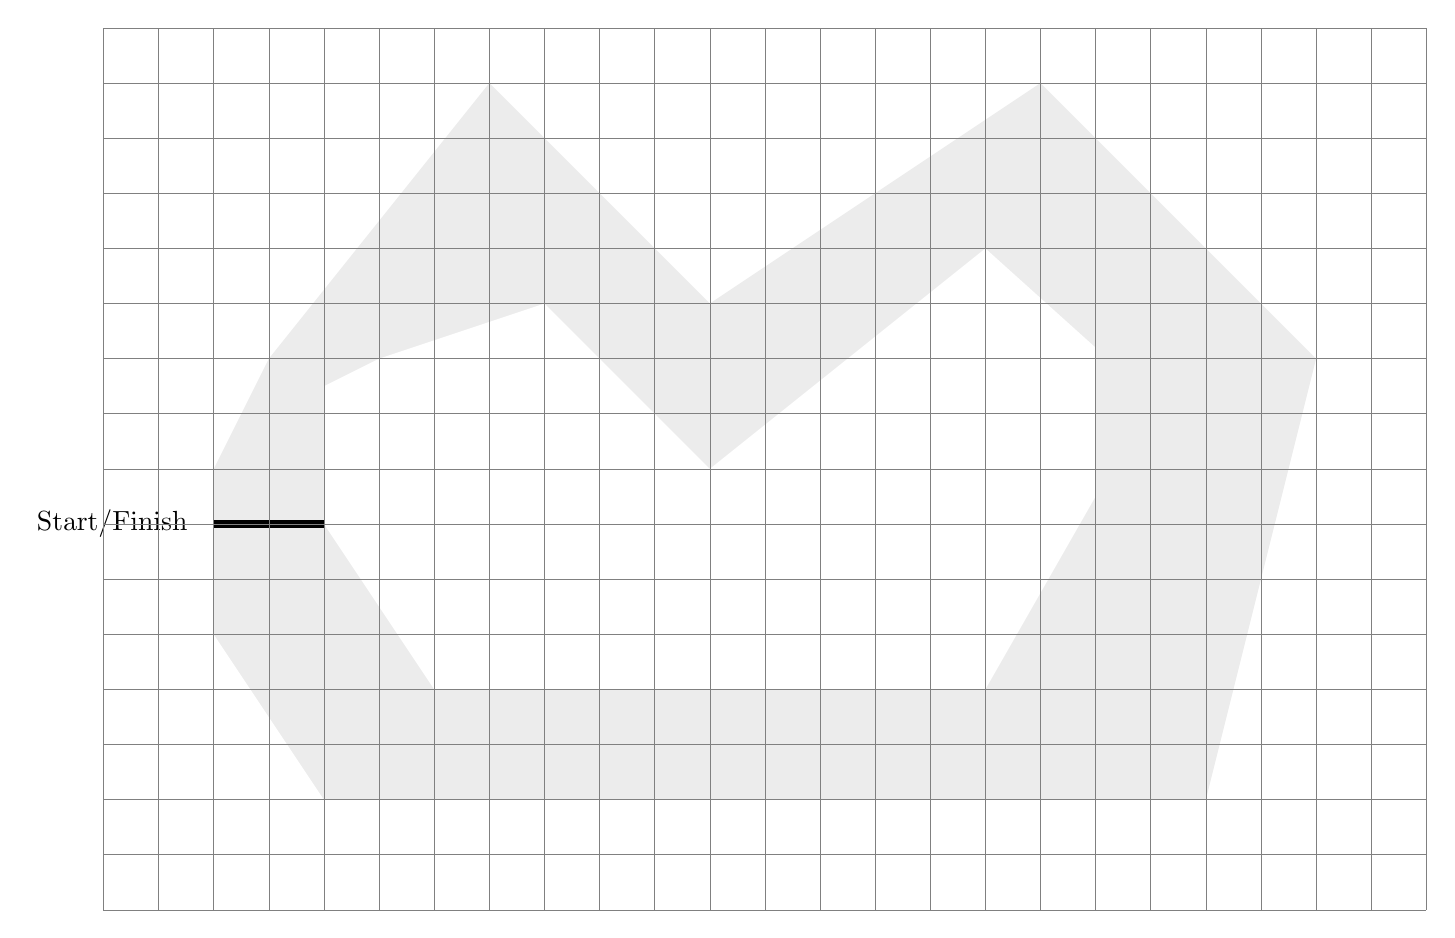
\begin{tikzpicture}[scale=0.7]
    % Grid underneath everything

    % --- Inner boundary (moved inward -> wider track) ---
    % Shifted inward by approx 2 units everywhere
    \draw[line width=3pt, rounded corners=26pt]
        (-8,-1)
        -- (-6,-4)
        -- (3,-4)
        -- (3,-2.5)
        -- (6,2.2)
        -- (3.2,4)
        -- (-1,2)
        -- (-4,4)
        -- (-7,2)
        -- (-8,1.5)
        -- cycle;

    % --- Fill the track band lightly, but keep grid visible ---
    \begin{scope}
        % Clip to the outer boundary
        \clip (-10,-3)
            -- (-8,-6)
            -- (8,-6)
            -- (9,-2)
            -- (10,2)
            -- (5,7)
            -- (-1,3)
            -- (-5,7)
            -- (-9,2)
            -- (-10,0)
            -- cycle;

        % Fill track band
        \fill[gray!15] (-12,-8) rectangle (12,8);

        % Punch out widened inner track
        \fill[white]
            (-8,-1)
            -- (-6,-4)
            -- (4,-4)
            -- (6,-0.5)
            -- (6,2.2)
            -- (4,4)
            -- (-1,0)
            -- (-4,3)
            -- (-7,2)
            -- (-8,1.5)
            -- cycle;
    \end{scope}
    % Start/Finish line
    \draw[line width=3pt] (-10,-1) -- (-8,-1);
    \node[anchor=east] at (-10.3,-1) {Start/Finish};

    \draw[help lines, step=1] (-12,-8) grid (12,8);

\end{tikzpicture}
\end{center}

\begin{center}
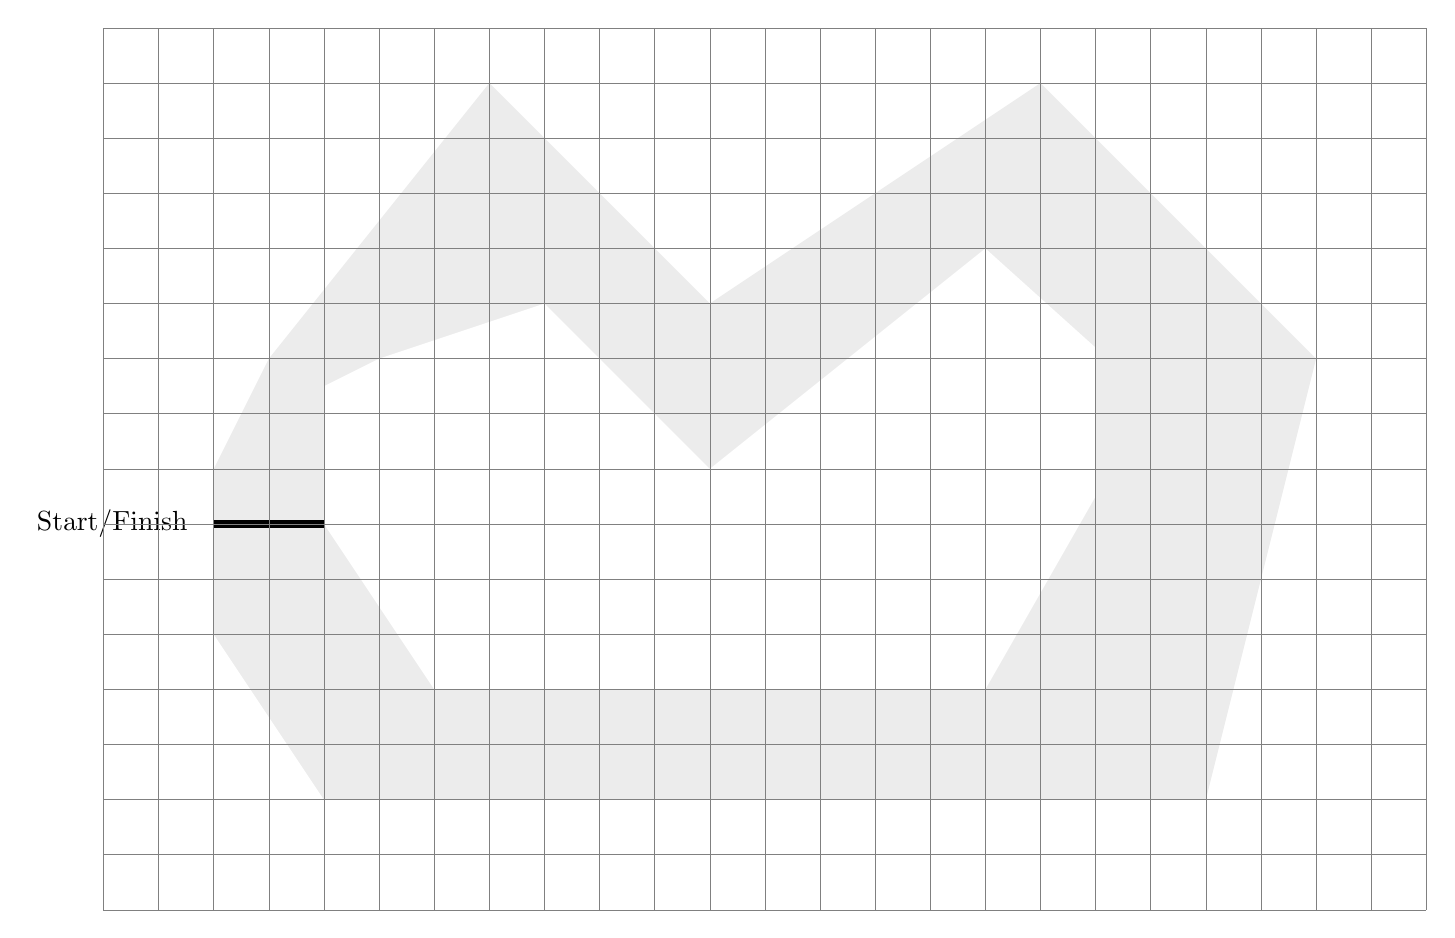
\begin{tikzpicture}[scale=0.7]
    % Grid underneath everything

    % --- Inner boundary (moved inward -> wider track) ---
    % Shifted inward by approx 2 units everywhere
    \draw[line width=3pt, rounded corners=26pt]
        (-8,-1)
        -- (-6,-4)
        -- (3,-4)
        -- (3,-2.5)
        -- (6,2.2)
        -- (3.2,4)
        -- (-1,2)
        -- (-4,4)
        -- (-7,2)
        -- (-8,1.5)
        -- cycle;

    % --- Fill the track band lightly, but keep grid visible ---
    \begin{scope}
        % Clip to the outer boundary
        \clip (-10,-3)
            -- (-8,-6)
            -- (8,-6)
            -- (9,-2)
            -- (10,2)
            -- (5,7)
            -- (-1,3)
            -- (-5,7)
            -- (-9,2)
            -- (-10,0)
            -- cycle;

        % Fill track band
        \fill[gray!15] (-12,-8) rectangle (12,8);

        % Punch out widened inner track
        \fill[white]
            (-8,-1)
            -- (-6,-4)
            -- (4,-4)
            -- (6,-0.5)
            -- (6,2.2)
            -- (4,4)
            -- (-1,0)
            -- (-4,3)
            -- (-7,2)
            -- (-8,1.5)
            -- cycle;
    \end{scope}
    % Start/Finish line
    \draw[line width=3pt] (-10,-1) -- (-8,-1);
    \node[anchor=east] at (-10.3,-1) {Start/Finish};

    \draw[help lines, step=1] (-12,-8) grid (12,8);

\end{tikzpicture}
\end{center}

\newpage{} 

\begin{enumerate}
    \item \ealpara{Napisz swoją ścieżkę w następującej postaci: \(g + a + ...\)}{Write your path in the following form: \(g + a + ...\)}
    \vspace{4em}
    \item \ealpara{Zbierz \ealkeytr{wyrazy podobne} w swoim \ealkeytr{wyrażeniu}}{Collect the \ealkey{like terms} in your \ealkey{expression}}
   \vspace{4em}
   \item \ealpara{Zatem \ealkeytr{oblicz} \ealkeytr{wyrażenie} z 1. jako \ealkeytr{wektor kolumnowy}; co zauważasz?}{Thus \ealkey{evaluate} the \ealkey{expression} from 1. as a \ealkey{column vector}, what do you notice?}

\end{enumerate}

\newpage{}

\begin{center}
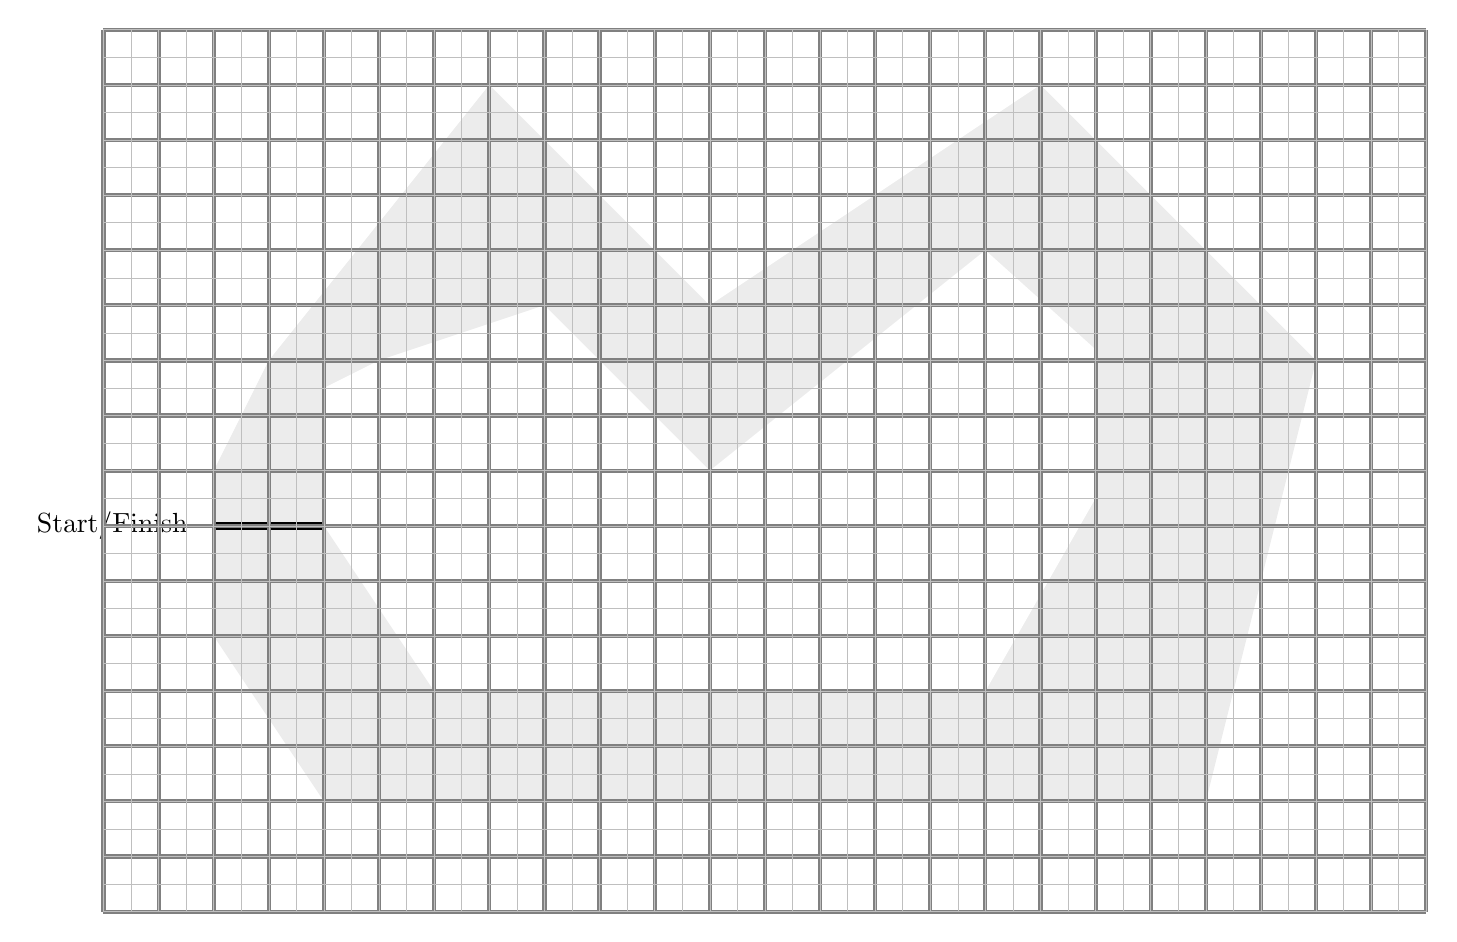
\begin{tikzpicture}[scale=0.7]
    % Grid underneath everything

    % --- Inner boundary (moved inward -> wider track) ---
    % Shifted inward by approx 2 units everywhere
    \draw[line width=3pt, rounded corners=26pt]
        (-8,-1)
        -- (-6,-4)
        -- (3,-4)
        -- (3,-2.5)
        -- (6,2.2)
        -- (3.2,4)
        -- (-1,2)
        -- (-4,4)
        -- (-7,2)
        -- (-8,1.5)
        -- cycle;

    % --- Fill the track band lightly, but keep grid visible ---
    \begin{scope}
        % Clip to the outer boundary
        \clip (-10,-3)
            -- (-8,-6)
            -- (8,-6)
            -- (9,-2)
            -- (10,2)
            -- (5,7)
            -- (-1,3)
            -- (-5,7)
            -- (-9,2)
            -- (-10,0)
            -- cycle;

        % Fill track band
        \fill[gray!15] (-12,-8) rectangle (12,8);

        % Punch out widened inner track
        \fill[white]
            (-8,-1)
            -- (-6,-4)
            -- (4,-4)
            -- (6,-0.5)
            -- (6,2.2)
            -- (4,4)
            -- (-1,0)
            -- (-4,3)
            -- (-7,2)
            -- (-8,1.5)
            -- cycle;
    \end{scope}
    % Start/Finish line
    \draw[line width=3pt] (-10,-1) -- (-8,-1);
    \node[anchor=east] at (-10.3,-1) {Start/Finish};

    \draw[help lines, step=1, line width=1.5pt] (-12,-8) grid (12,8);
    \draw[step=0.5, help lines, color=gray!50] (-12,-8) grid (12,8);


\end{tikzpicture}
\end{center}


\begin{center}
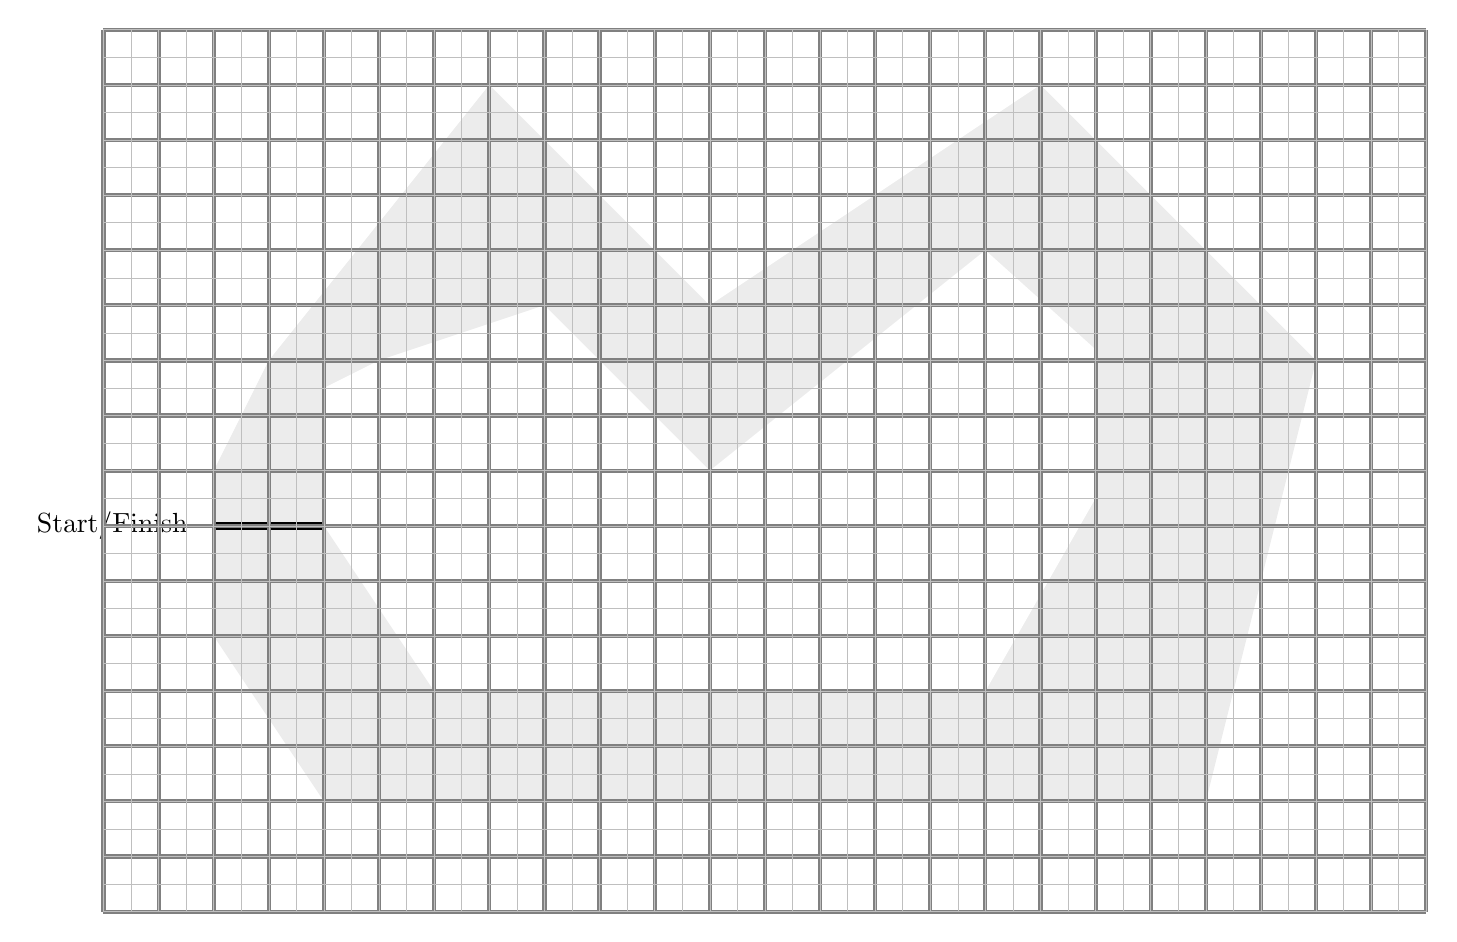
\begin{tikzpicture}[scale=0.7]
    % Grid underneath everything

    % --- Inner boundary (moved inward -> wider track) ---
    % Shifted inward by approx 2 units everywhere
    \draw[line width=3pt, rounded corners=26pt]
        (-8,-1)
        -- (-6,-4)
        -- (3,-4)
        -- (3,-2.5)
        -- (6,2.2)
        -- (3.2,4)
        -- (-1,2)
        -- (-4,4)
        -- (-7,2)
        -- (-8,1.5)
        -- cycle;

    % --- Fill the track band lightly, but keep grid visible ---
    \begin{scope}
        % Clip to the outer boundary
        \clip (-10,-3)
            -- (-8,-6)
            -- (8,-6)
            -- (9,-2)
            -- (10,2)
            -- (5,7)
            -- (-1,3)
            -- (-5,7)
            -- (-9,2)
            -- (-10,0)
            -- cycle;

        % Fill track band
        \fill[gray!15] (-12,-8) rectangle (12,8);

        % Punch out widened inner track
        \fill[white]
            (-8,-1)
            -- (-6,-4)
            -- (4,-4)
            -- (6,-0.5)
            -- (6,2.2)
            -- (4,4)
            -- (-1,0)
            -- (-4,3)
            -- (-7,2)
            -- (-8,1.5)
            -- cycle;
    \end{scope}
    % Start/Finish line
    \draw[line width=3pt] (-10,-1) -- (-8,-1);
    \node[anchor=east] at (-10.3,-1) {Start/Finish};

    \draw[help lines, step=1, line width=1.5pt] (-12,-8) grid (12,8);
    \draw[step=0.5, help lines, color=gray!50] (-12,-8) grid (12,8);

\end{tikzpicture}
\end{center}



\newpage{}


\begin{center}
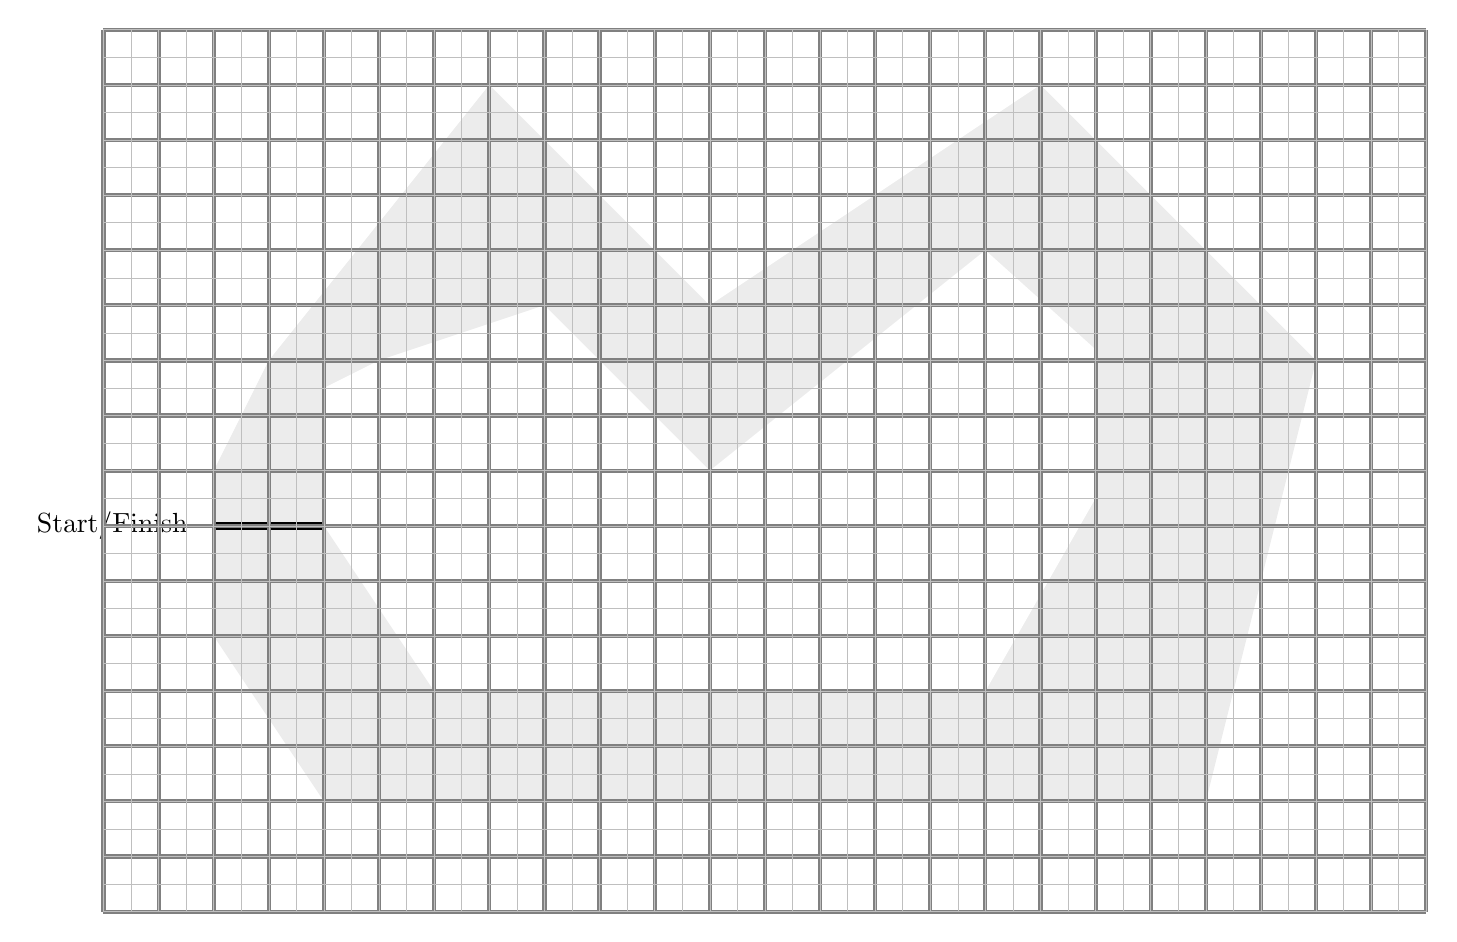
\begin{tikzpicture}[scale=0.7]
    % Grid underneath everything

    % --- Inner boundary (moved inward -> wider track) ---
    % Shifted inward by approx 2 units everywhere
    \draw[line width=3pt, rounded corners=26pt]
        (-8,-1)
        -- (-6,-4)
        -- (3,-4)
        -- (3,-2.5)
        -- (6,2.2)
        -- (3.2,4)
        -- (-1,2)
        -- (-4,4)
        -- (-7,2)
        -- (-8,1.5)
        -- cycle;

    % --- Fill the track band lightly, but keep grid visible ---
    \begin{scope}
        % Clip to the outer boundary
        \clip (-10,-3)
            -- (-8,-6)
            -- (8,-6)
            -- (9,-2)
            -- (10,2)
            -- (5,7)
            -- (-1,3)
            -- (-5,7)
            -- (-9,2)
            -- (-10,0)
            -- cycle;

        % Fill track band
        \fill[gray!15] (-12,-8) rectangle (12,8);

        % Punch out widened inner track
        \fill[white]
            (-8,-1)
            -- (-6,-4)
            -- (4,-4)
            -- (6,-0.5)
            -- (6,2.2)
            -- (4,4)
            -- (-1,0)
            -- (-4,3)
            -- (-7,2)
            -- (-8,1.5)
            -- cycle;
    \end{scope}
    % Start/Finish line
    \draw[line width=3pt] (-10,-1) -- (-8,-1);
    \node[anchor=east] at (-10.3,-1) {Start/Finish};

    \draw[help lines, step=1, line width=1.5pt] (-12,-8) grid (12,8);
    \draw[step=0.5, help lines, color=gray!50] (-12,-8) grid (12,8);

\end{tikzpicture}
\end{center}

\begin{center}
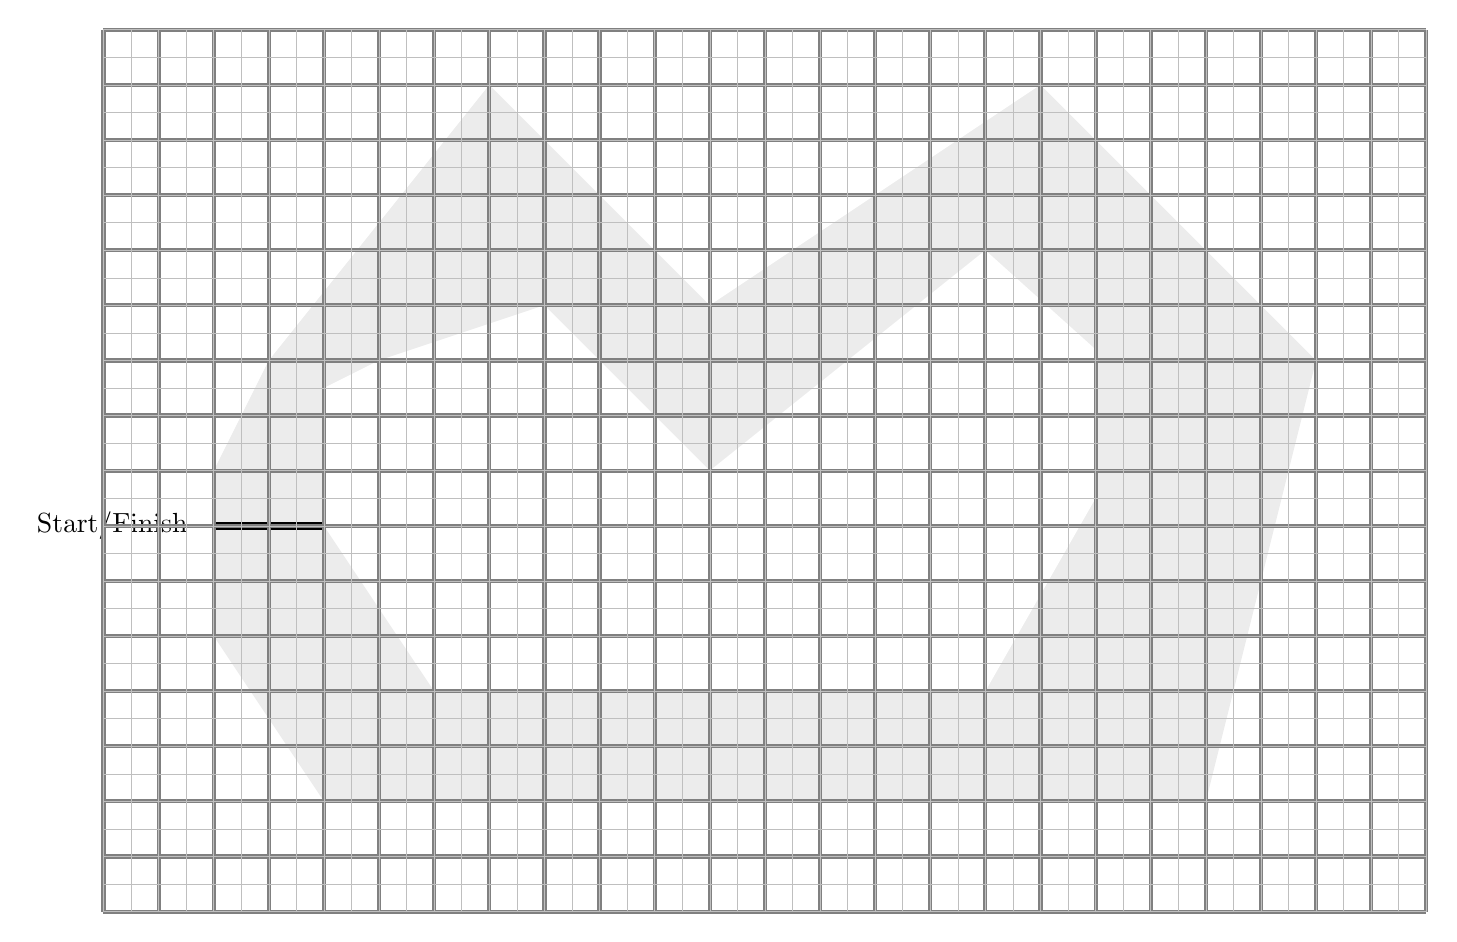
\begin{tikzpicture}[scale=0.7]
    % Grid underneath everything

    % --- Inner boundary (moved inward -> wider track) ---
    % Shifted inward by approx 2 units everywhere
    \draw[line width=3pt, rounded corners=26pt]
        (-8,-1)
        -- (-6,-4)
        -- (3,-4)
        -- (3,-2.5)
        -- (6,2.2)
        -- (3.2,4)
        -- (-1,2)
        -- (-4,4)
        -- (-7,2)
        -- (-8,1.5)
        -- cycle;

    % --- Fill the track band lightly, but keep grid visible ---
    \begin{scope}
        % Clip to the outer boundary
        \clip (-10,-3)
            -- (-8,-6)
            -- (8,-6)
            -- (9,-2)
            -- (10,2)
            -- (5,7)
            -- (-1,3)
            -- (-5,7)
            -- (-9,2)
            -- (-10,0)
            -- cycle;

        % Fill track band
        \fill[gray!15] (-12,-8) rectangle (12,8);

        % Punch out widened inner track
        \fill[white]
            (-8,-1)
            -- (-6,-4)
            -- (4,-4)
            -- (6,-0.5)
            -- (6,2.2)
            -- (4,4)
            -- (-1,0)
            -- (-4,3)
            -- (-7,2)
            -- (-8,1.5)
            -- cycle;
    \end{scope}
    % Start/Finish line
    \draw[line width=3pt] (-10,-1) -- (-8,-1);
    \node[anchor=east] at (-10.3,-1) {Start/Finish};

    \draw[help lines, step=1, line width=1.5pt] (-12,-8) grid (12,8);
    \draw[step=0.5, help lines, color=gray!50] (-12,-8) grid (12,8);

\end{tikzpicture}
\end{center}


\end{document}